\subsection{Who}

\begin{frame}{\myframetitle}
	\begin{mycolumns}
		\only<1|handout:1>{
			\begin{example}{Who Are You? \mysource{\universitycourses} \tiny ;-)}
				\centering
				\small
				\featureDiagram{
					You,concrete
						[Degree,concrete,mandatory
							[Bachelor,concrete,alternative]
							[Master,concrete]]
						[WPF,concrete,mandatory]
						[Interest,concrete,mandatory]
						[Course,concrete,mandatory
							[INF,concrete,alternative]
							[CV,concrete]
							[WIF,concrete]
							[INGIF,concrete]
							[DE,concrete]]
				}\\[1ex]
				$\textsf{Bachelor} \pimplies \textsf{ECTS} = 5$\\
				$\textsf{Master} \pimplies \textsf{ECTS} = 6$
			\end{example}
		}
		\only<2-|handout:2>{
			\begin{example}{Who Are You?}
				\begin{itemize}
					\item a \emph{Bachelor student} (5 ECTS) or
					\item a \emph{Master student} (6 ECTS)
					\item looking for an \emph{elective subject} \deutsch{Wahlpflichtfach (WPF)}
					\item enrolled in \emph{INF}, \emph{CV}, \emph{WIF}, \emph{INGIF}, or \emph{DE}
					\item interested in
					\begin{itemize}
						\item \emph{learning} about the basic principles of systematically managing software variability
						\item \emph{experimenting} with novel software engineering methods and tools
						\item getting in touch with current \emph{research} on software product lines
					\end{itemize}
				\end{itemize}
			\end{example}
		}
		\mynextcolumn
		\only<3-|handout:2>{
			\begin{note}{Who Are We?}
				\centering
				\parbox{0.45\linewidth}{
					\centering
					\href{https://www.dbse.ovgu.de/Mitarbeiter/Gunter+Saake.html}{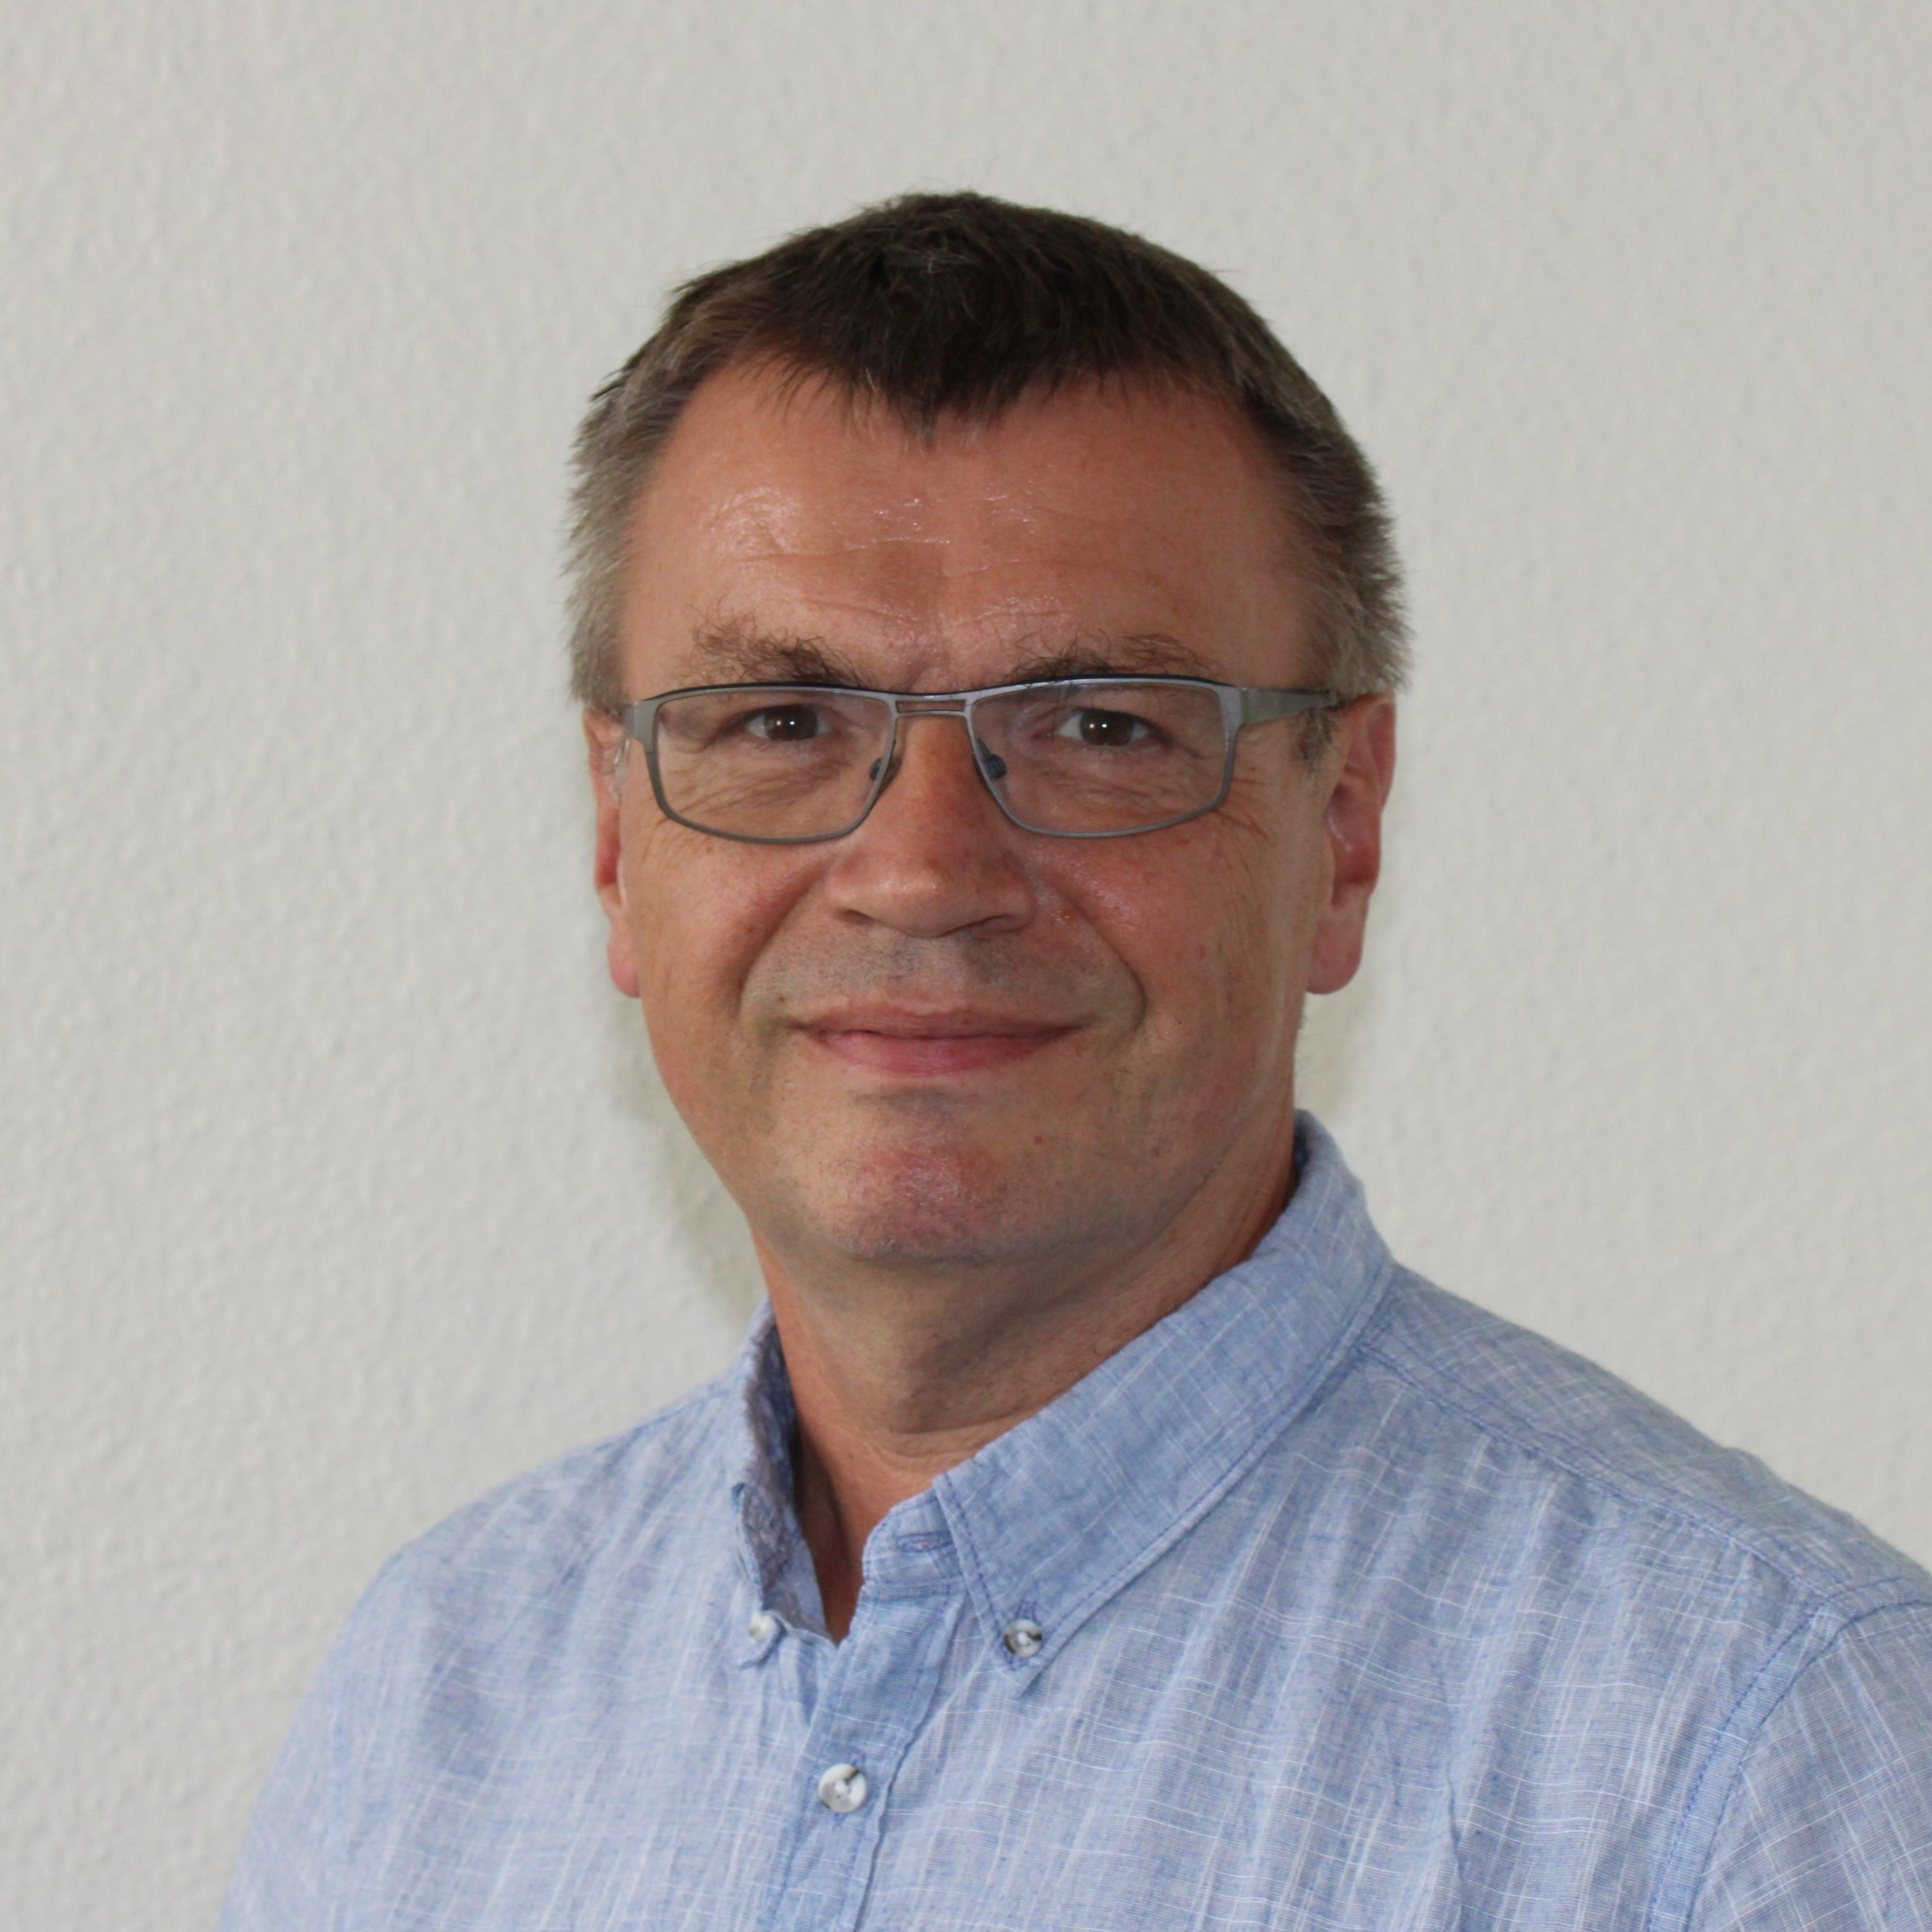
\includegraphics[width=\linewidth]{gunter-saake}}\\[.5ex]
					\href{https://www.dbse.ovgu.de/Mitarbeiter/Gunter+Saake.html}{\emph{Gunter Saake}}\\[.5ex]
					\small professor for databases and software engineering\\[.5ex]
					FeatureIDE project manager
				}
				\parbox{0.45\linewidth}{
					\centering
					\href{https://www.dbse.ovgu.de/Mitarbeiter/Elias+Kuiter.html}{
\includegraphics[width=0.75\linewidth]{elias-kuiter}}\\[.5ex]
					\href{https://www.dbse.ovgu.de/Mitarbeiter/Elias+Kuiter.html}{\emph{Elias Kuiter}}\\[.5ex]
					\small PhD student in feature-model analysis\\[.5ex]
					FeatureIDE core developer
				}
			\end{note}
		}
	\end{mycolumns}
\end{frame}

\subsection{Where and When}

\begin{frame}{\myframetitle}
	\begin{mycolumns}
		\begin{definition}{Lecture}
			\begin{itemize}
				\item once per week (2 SWS)
				\begin{itemize}
					\item on \emph{Friday}, 09.15am--10.45am
					\item in room G22A-122
					\item starts on October 13
				\end{itemize}
				\item held by Gunter + Elias + guests
				\item \emph{slides} are available on \texttt{\href{https://elearning.ovgu.de/course/view.php?id=15521}{Moodle}}
				\item \emph{guest lectures} planned:
				\begin{itemize}
					\item industry talk around Christmas
					\item research talks at end of January
				\end{itemize}
			\end{itemize}
		\end{definition}
	\mynextcolumn
		\begin{example}{Exercise}
			\begin{itemize}
				\item once per week (2 SWS)
				\begin{itemize}
					\item on \emph{Tuesday}, 09.15am--10.45am
					\item in room G05-117
					\item starts on October 17
				\end{itemize}
				\item held by Elias
				\item exercise sheets are available on \texttt{\href{https://elearning.ovgu.de/course/view.php?id=15521}{Moodle}}
				\begin{itemize}
					\item \emph{homework tasks} on each exercise sheet
					\item \emph{practical tasks} every two weeks, worked on in teams of $2$--$3$ students
				\end{itemize}
			\end{itemize}
		\end{example}
	\end{mycolumns}
\end{frame}

\subsection{Taking the Exam, and Beyond}

\begin{frame}{\myframetitle}
	\begin{mycolumns}
		\begin{definition}{Exam Eligibility \deutsch{Prüfungszulassung}}
			\begin{itemize}
				\item 60\% of all normal tasks \deutsch{Votierungspunkte}
				\item 70\% for Master students
				\item 4 presentation points \deutsch{Vortragspunkte}
				\item all practical tasks
			\end{itemize}
		\end{definition}
	\mynextcolumn
		\begin{definition}{Exam}
			\begin{itemize}
				\item oral exam ($\approx 20$ minutes)
				\item 1--2 exam days in February or March
				\item to get an ungraded performance \deutsch{Schein}, you have to pass the exam
			\end{itemize}
		\end{definition}
		\begin{example}{Further Studies}
			\begin{itemize}
				\item \emph{Individual Project, Software Project}
				\item \emph{Master Thesis} (several open topics on SPLE)
				\item \emph{PhD Thesis?} (SPLs are still actively researched)
			\end{itemize}
			\ldots{} contact us!
		\end{example}
	\end{mycolumns}
\end{frame}
